%% This document is created by 
%%  Dr. Putu Harry Gunawan
%% Template untuk Proposal TA 1 dan TA
%% Template ini digunakan untuk penulisan proposal TA 1 atau TA Fakultas Informatika, Telkom University.

\documentclass[a4paper,12pt,oneside]{book}

\setcounter{tocdepth}{5}
\setcounter{secnumdepth}{5}

\usepackage{hyperref}

\usepackage[utf8]{inputenc}
\usepackage{sectsty}
\usepackage{graphicx}
\usepackage{epstopdf}
\usepackage{algorithm}
\usepackage[table]{xcolor}
\usepackage{algpseudocode}
\usepackage{array}
%\usepackage[dvipsnames]{xcolor}
\usepackage{anysize}
\usepackage{amsmath}
\usepackage{amssymb}
\usepackage[bahasa]{babel}
\usepackage{indentfirst} %Spasi untuk paragraf pertama
\usepackage{geometry}
\usepackage{multirow}% http://ctan.org/pkg/multirow
\usepackage{hhline}% http://ctan.org/pkg/hhline
\marginsize{4cm}{3cm}{3cm}{3cm} %{left}{right}{top}{bottom}
\usepackage[compact]{titlesec} 
\usepackage{etoolbox}
\usepackage{theorem}
\usepackage{comment}
\usepackage{verbatim}
\newtheorem{definition}{Definisi}
\newtheorem{catatan}{Catatan}
\newtheorem{theorem}{Teorema}
\newtheorem{lemma}{Lema}
\newtheorem{spec}{Spesifikasi}
\floatname{algorithm}{Skrip NuSMV}
\newenvironment{proof}[1][Bukti]{\noindent\textsc{#1:} }{\hfill$\square$}

\hyphenation{me-la-ku-kan}

\makeatletter
\patchcmd{\ttlh@hang}{\parindent\z@}{\parindent\z@\leavevmode}{}{}
\patchcmd{\ttlh@hang}{\noindent}{}{}{}
\makeatother

\chapterfont{\centering}
\newcommand{\bigsize}{\fontsize{16pt}{14pt}\selectfont}
\chapterfont{\centering\bigsize\bfseries}
\sectionfont{\large\bfseries}
\usepackage{tikz}
\usetikzlibrary{shapes.geometric, arrows}
%\renewcommand{\chaptertitle}{BAB}
\renewcommand{\thechapter}{\Roman{chapter}}
\renewcommand\thesection{\arabic{chapter}.\arabic{section}}
\renewcommand\thesubsection{\thesection.\arabic{subsection}}
\renewcommand{\theequation}{\arabic{chapter}.\arabic{equation}}
\renewcommand{\thefigure}{\arabic{chapter}.\arabic{figure}}
\renewcommand{\thetable}{\arabic{chapter}.\arabic{table}}

\renewcommand\bibname{Daftar Pustaka}
\addto{\captionsbahasa}{\renewcommand{\bibname}{Daftar Pustaka}}
\usepackage{fancyhdr}
\pagestyle{fancy}
\lhead{}
\chead{}
\rhead{}
\lfoot{}
\cfoot{\thepage}
\rfoot{}
\renewcommand{\headrulewidth}{0pt}

\makeatletter

%%%%%%%%%%%%%%%%%%%%%%%%%%%%%%%%%%%%%%%%%%%%%%%%%%%%%%%%%%%%
%
%  Berikut adalah data-data yang wajib diisi oleh mahasiswa
%
%%%%%%%%%%%%%%%%%%%%%%%%%%%%%%%%%%%%%%%%%%%%%%%%%%%%%%%%%%%%

\title{Pemecah Sudoku Interaktif Dengan Logika Proposisi}\let\Title\@title   %Judul dalam bahasa Indonesia

\newcommand{\EngTitle}{Interactive Sudoku Solver Using Propositional Logic}  %Judul dalam bahasa Inggris

\author{Muhammad Zakaria Musa}  \let\Author\@author  %Nama mhs
\newcommand{\NIM}{1103130047}
\newcommand{\Prodi}{Teknik Informatika}
\newcommand{\KK}{\textit{Intelligence, Computing, and Multimedia}} %UNTUK TA
\newcommand{\Gelar}{} % UNTUK TA
\date{2017}           \let\Date\@date %Maskkan hanya tahun saja
\newcommand{\Tanggal}{24} % Tanggal Pengesahan
\newcommand{\Bulan}{November} % Bulan Pengesahan
\newcommand{\PembimbingSatu}{Yanti Rusmawati, Ph.D.}
\newcommand{\NIPPembimbingSatu}{15711785-1}
\newcommand{\PembimbingDua}{Muhammad Arzaki, M.Kom.}
\newcommand{\NIPPembimbingDua}{15871701-2}
\newcommand{\Kaprodi}{Moch. Arif Bijaksana, Ph.D.}
\newcommand{\NIPKaprodi}{03650312-4}
\newif\iflogTA
%\logTAtrue   %%%%%% WARNING kode ini diaktifkan untuk format TUGAS AKHIR
\makeatother
\linespread{1}


\begin{document}
\pagenumbering{roman} 
%%\maketitle
\begin{titlepage}
\thispagestyle{empty}
%\vspace*{0.7cm}
{\centering
\large
{\bigsize\bf \Title}\\
\vspace{ 2cm}
\rm
\iflogTA
\textbf{Tugas Akhir}\\
\vspace{0.5 cm}
\textbf{Kelompok Keahlian: \KK}\\
\else
\textbf{Proposal Tugas Akhir}\\
\vspace{0.5 cm}
\textbf{Kelas TA 1}\\
\fi
\vspace{0.5 cm}
\textbf{\Author}\\ \textbf{NIM: \NIM}\\ 

\vspace{1.5 cm}

\begin{figure}[h]
{\centering {
\includegraphics[scale=0.17]{Tel-U-Logo}}\par}
\end{figure}

\vspace{2 cm}
{\bigsize\textbf{Program Studi Sarjana \Prodi}\\
\vspace{0.5 cm}
\textbf{Fakultas Informatika}\\
\vspace{0.5 cm}
\textbf{Universitas Telkom}\\
\vspace{0.5 cm}
\textbf{Bandung}\\
\vspace{0.5 cm}
\textbf{\Date}\\}
}
\pagebreak
\iflogTA
\chapter*{Lembar Pernyataan}

Saya yang bertanda tangan dbawah ini:

Nama \qquad : \qquad 

NIM  \qquad  : \qquad 

Menyatakan bahwa Tugas Akhir dengan judul . . . .
merupakan karya orisinil saya sendiri, ditulis dengan tidak menjiplak karya orang lain, mengutip
dengan cara-cara yang sesuai dengan etika keilmuan yang berlaku dalam masyarakat keilmuan.
Atas pernyataan ini saya siap menanggung resiko atau sanksi yang dijatuhkan kepada saya
apabila kemudian ditemukan adanya pelanggaran terhadap kejujuran akademik ataupun etika
keilmuan dalam Tugas Akhir ini, atau ditemukan bukti yang menunjukan ketidak aslian karya
ini.

\hfill

\hfill Bandung

\hfill Yang membuat pernyataan

\hfill

\hfill

\hfill

\hfill

\hfill

\hfill <nama>

\hfill <nim>
\pagebreak
\fi
\thispagestyle{empty}
{\centering
\iflogTA
\textbf{\large Lembar Pengesahan}\\  %UNTUK TA
\else
\textbf{\large Lembar Persetujuan}\\
\fi
\vspace{0.5cm}
\textbf{\Title}\\
\vspace{0.5cm}
\textbf{\textit{\EngTitle}}\\
\vspace{0.5cm}
\textbf{\Author}\\
\textbf{NIM: \NIM}\\
\vspace{1cm}

\iflogTA 
{ Tugas Akhir ini diterima dan disahkan untuk memenuhi sebagian dari syarat untuk memperoleh gelar sarjana \Gelar\\ Program Studi Sarjana \Prodi\\ Fakultas Informatika Universitas Telkom}\\  %% UNTUK TA
\else
{ Proposal ini diajukan sebagai usulan pembuatan tugas akhir pada\\ Program Studi Sarjana \Prodi\\ Fakultas Informatika Universitas Telkom}\\
\fi
\vspace{0.5cm}

{Bandung, \Tanggal\quad \Bulan \quad \Date}\\
{Menyetujui}\\

\vspace{0.5cm}
\iflogTA
\begin{center}
\begin{tabular}{  m{8cm}  m{8cm} }
Pembimbing 1 & Pembimbing 2
\end{tabular}
\end{center}
\else
\begin{center}
\begin{tabular}{  m{8cm}  m{8cm} }
Calon Pembimbing 1 & Calon Pembimbing 2
\end{tabular}
\end{center}
\fi
\begin{center}
\vspace{2cm}
\begin{tabular}{  m{8cm}  m{8cm} }
\underline{\PembimbingSatu} & \underline{\PembimbingDua} \\ 
NIP: \NIPPembimbingSatu & NIP: \NIPPembimbingDua
\end{tabular}
\end{center}
\vspace{0.5cm}
\iflogTA
Mengesahkan,\\   %% UNTUK TA
Kepala Program Studi \Prodi\\ %% UNTUK TA
\vspace{2.5cm}   %% UNTUK TA
\underline{\Kaprodi}\\ NIP: \NIPKaprodi\\  %% UNTUK TA
\fi
}
\pagebreak
\end{titlepage}
\addcontentsline{toc}{chapter}{Abstrak}
\chapter*{Abstrak}

Abstrak . . . .
  
\vspace{0.5 cm}
\begin{flushleft}
{\textbf{Kata Kunci:}  metode formal, SAT solver, Sudoku, pengujian kotak hitam . . . . }
\end{flushleft}
\iflogTA
\pagebreak
\addcontentsline{toc}{chapter}{Abstract}
\chapter*{Abstract}

Abstract . . . .

\vspace{0.5 cm}
\begin{flushleft}
{\textbf{Keywords:} formal method, SAT solver, sudoku, black box testing . . . . }
\end{flushleft}
\pagebreak
\addcontentsline{toc}{chapter}{Lembar Persembahan}
\chapter*{Lembar Persembahan}

  \textit{Alhamdulillah}, Puji dan syukur saya panjatkan kepada Allah SWT karena atas petunjuk dan ridha-Nya lah penulis dapat menyelesaikan tugas akhir ini. Pada kesempatan ini penulis ingin menyampaikan rasa terima kasih kepada pihak-pihak yang telah membantu penulis selama ini:
  \begin{enumerate}
      \item Kepada Tuhan Yang Maha Esa, atas berkat dan rahmat-Nya tugas akhir ini dapat dikerjakan dengan lancar.
      
      \item Kepada Kedua Orangtua saya, terima kasih atas doa dan dukungannya selama ini.
      
      \item Kepada Bu Yanti dan Pak Arzaki, terima kasih atas ilmu dan bantuannya selama ini.
      
      \item Kepada Sarah dan Kak Damar, terima kasih atas bantuannya selama ini.
      
      \item Kepada Teman-teman saya, baik teman kelas, kontrakan, kosan, dan Nihon no Matsuri, terima kasih dukungannya.
      
      \item Kepada Lab Computing, terima kasih sudah memberikan tempat selama pengerjaan penelitian ini.
      
      \item Kepada pihak-pihak lain yang tidak dapat dituliskan satu persatu.
  \end{enumerate}
\pagebreak
\addcontentsline{toc}{chapter}{Kata Pengantar}
\chapter*{Kata Pengantar}

Segala puji dan syukur saya panjatkan kepada Allah SWT, karena ridha-Nya lah penulis dapat menyelesaikan penelitian tugas akhir yang berjudul ``Verifikasi Alur Distribusi Vaksin di Indonesia menggunakan Logika Temporal Linear" sebagai salah satu syarat untuk mendapatkan gelar sarjana di Universitas Telkom. Penelitian ini membahas tentang pemodelan formal dari alur distribusi vaksin di Indonesia dengan bahasa logika tertentu. Hasil dari penelitian ini diharapkan memberikan manfaat untuk PT. Bio Farma dan para pembaca. Terima kasih penulis ucapkan untuk para pembaca.\\\\\\Bandung, 28 Agustus 2017
\\
Penulis
\\
\\
\\
\\
(Muhammad Zakaria Musa)
\pagebreak
\fi
\cleardoublepage
\addcontentsline{toc}{chapter}{Daftar Isi}
\tableofcontents
\iflogTA
\newpage
\cleardoublepage
\addcontentsline{toc}{chapter}{Daftar Gambar}
\listoffigures
\newpage
\cleardoublepage
\addcontentsline{toc}{chapter}{Daftar Tabel}
\listoftables
%\pagebreak
\fi
%
\cleardoublepage
\pagenumbering{arabic}
\chapter{Pendahuluan}

\section{Latar Belakang}

Pada Tahun 2015 \textit{The Organization for Economic Co-operation and Development}(OECD) merilis nilai dari \textit{Programme for International Student Assessment}(PISA). Yang merupakan nilai kemampuan siswa pada matematika, membaca, dan membaca. Pada kategori matematika Indosnesia menempati peringkat 65 dari 71 negara dengan nilai 386. Sedangkan nilai rata-rata OECD untuk matematika adalah 470. Hal ini sungguh memprihatinkan. Oleh karena itu diperlukan katalis yang dapat mengembangkan kemampuan \textit{logical thinking} serta \textit{problem solving} anak salah satunya adalah dengan sudoku. 

Sudoku berasal dari kata \textit{Sūji wa dokushin ni kagiru} yang berarti angkanya harus tunggal \cite{SATPy3} adalah suatu \textit{puzzle} (teka-teki) yang direpresentasikan oleh sebuah matriks (\textit{array}
dua dimensi) berukuran ${n^2 \times n^2}$  yang dibangun dari ${n^2}$ dengan submatriks (atau blok)
yang berukuran ${n \times n}$. Sudoku merupakan \textit{puzzle}
yang biasanya dimainkan oleh satu orang.  Pada
awal permainan, terdapat beberapa sel yang telah terisi yang disebut dengan pemberian
(\textit{givens}). Untuk menyelesaikan permainan ini, seorang pemain harus mengisi setiap sel yang
belum terisi dengan angka di antara 1 sampai
$n^2$ sedemikan sehingga setiap baris, setiap kolom,
dan setiap blok (submatriks berukuran $n \times n$) memuat tepat satu bilangan di antara 1 sampai $n^2$. Biasanya suatu sudoku didesain agar tepat memiliki satu kemungkinan solusi. Hal
ini juga mengakibatkan sudoku dapat diselesaikan hanya dengan mengandalkan penalaran
yang sederhana. Pengisian suatu sel dapat dilakukan dengan meninjau kemungkinan dari
isi sebuah sel.

Banyak pemain yang terjebak pada teka-teki sudoku dan tidak dapat melanjutkan permainan. Hal ini terjadi karena pemain mengisi nilai yang salah atau sudoku tidak memiliki solusi. Oleh karena itu banyak pemain yang membutuhkan pemecah sudoku yang dapat memberikan keterpenuhan dari sebuah sudoku. Sehingga pemain dapat mengetahui sebuah sudoku memiliki solusi atau tidak.

Hingga saat ini, sudah banyak penelitian yang membahas penyelesaian sudoku secara
matematis maupun komputasional. Salah satu metode yang cukup dikenal adalah penyelesaian
sudoku dengan memanfaatkan masalah keterpenuhan formula proposisional (\textit{propositional satisfiability problem}). Dengan pendekataan ini, syarat-syarat yang
harus dipenuhi oleh suatu sudoku dimodelkan dengan satu atau lebih formula logika proposisi \cite{KJ06,LO06}.
Keterpenuhan (\textit{satisfiability}) dari himpunan formula yang memodelkan syarat-syarat
ini akan menjamin bahwa suatu sudoku memiliki suatu solusi.

Pada tugas akhir ini, penulis akan membuat pemecah sudoku interaktif berbasis python. Bahasa python dipilih
karena implementasi SAT solver dalam bahasa python masih masih sedikit dibandingkan pada bahasa C dan C++ \cite{SATPy1}. Aplikasi akan menggunakan pengujian kotak hitam untuk menilai kualitas aplikasi \cite{TEST1}.

\section{Perumusan Masalah}

Berdasarkan latar belakang tersebut, rumusan masalah pada tugas akhir ini
adalah bagaimana cara membuat SAT solver bebasis python untuk pemecah sudoku yang interaktif.

\section{Batasan Masalah}

Batasan pada tugas akhir ini terbatas pada:
\begin{enumerate}
	\item Penulis hanya membangun aplikasi sudoku solver berukuran ($4\times4$), ($9\times9$), ($16\times16$).
	\item Untuk setiap ukuran sudoku memiliki tiga tingkat kesulitan. Yaitu mudah, menengah, sulit.
	\item Program mengeluarkan keterpenuhan dari sudoku.
	\item Program mengeluarkan solusi dari sudoku jika pengguna mengiginkan.
	\item Aplikasi akan diuji dengan metode
	pengujian kotak hitam (\textit{black box testing}).
\end{enumerate}

\section{Tujuan}

Tujuan yang ingin dicapai pada tugas akhir ini adalah untuk membuat pemecah sudoku yang interaktif.

\section{Rencana Kegiatan}

Pada pengerjaan tugas akhir ini beberapa hal yang akan saya lakukan adalah sebagai berikut:
\begin{enumerate}
	\item Analisa spesifikasi dan Kebutuhan sistem.
	\item Translasi spesifikasi sistem.
	\item Pembuatan aplikasi.
	\item Pengujian aplikasi.
	\item Analisis sistem.
	\item Penulisan laporan.
	
\end{enumerate}

\section{Jadwal Kegiatan}

Jadwal pengerjaan tugas akhir sesuai dengan alur yang telah dibuat.

\begin{table}[H]
	\caption{Jadwal Kegiatan.}
	
	\begin{center}
		\resizebox{\textwidth}{!}
		{\begin{tabular}{|c|p{5cm}|p{2cm}|p{2cm}|p{2cm}|p{2cm}|p{2cm}|p{2cm}|p{2cm}|}
				\hline 
				\multirow{2}{*}{No} & \multirow{2}{*}{Jenis Kegiatan} & \multicolumn{7}{c|}{Bulan}
				\tabularnewline
				
				\cline{3-9} 
				&  & November 2017 & Desember 2017 & Januari 2018 & Februari 2018 & Maret 2018 & April 2018 & Mei 2018
				\tabularnewline
				
				\hline 
				1 & Analisa spesifikasi dan kebutuhan sistem & \cellcolor{cyan} & \cellcolor{cyan} &  &  &  &  & \tabularnewline
				
				\hline 
				2 & Translasi spesifikasi sistem &  & \cellcolor{red} &  &  &  &  & \tabularnewline
				
				\hline 
				3 & Pembuatan aplikasi &&  
				\cellcolor{green} & \cellcolor{green} & \cellcolor{green} & \cellcolor{green} &  & \tabularnewline
				
				\hline 
				4 & Pengujian aplikasi &  &  &  &  & \cellcolor{darkgray} & \cellcolor{darkgray} & \tabularnewline
				
				\hline 
				5 & Analisis sistem &  &  &  &  &  & \cellcolor{lightgray} & \cellcolor{lightgray} \tabularnewline
				
				\hline 
				6 & Penulisan Laporan & \cellcolor{yellow} & \cellcolor{yellow} & \cellcolor{yellow} & \cellcolor{yellow} & \cellcolor{yellow} & \cellcolor{yellow} & \cellcolor{yellow} 
				\tabularnewline
				
				\hline 
		\end{tabular}}
		\par\end{center}
\end{table}
%
\chapter{Kajian Pustaka}

Pada bab ini penulis akan menjelaskan teori yang digunakan selama pengerjaan tugas akhir.

\section{Sudoku}

Sudoku berasal dari kata \textit{Sūji wa dokushin ni kagiru} yang berarti angkanya harus tunggal \cite{SATPy3}. Sudoku dipopulerkan di jepang oleh \textit{Nikoli in the paper Monthly Nikolist} pada April 1984. Sudoku adalah suatu \textit{puzzle} (teka-teki) yang direpresentasikan oleh sebuah matriks (\textit{array}
dua dimensi) berukuran ${n^2 \times n^2}$  yang dibangun dari ${n^2}$ dengan submatriks (atau blok)
yang berukuran ${n \times n}$. Sudoku merupakan \textit{puzzle}
yang biasanya dimainkan oleh satu orang.  Pada
awal permainan, terdapat beberapa sel yang telah terisi yang disebut dengan pemberian
(\textit{givens}). Untuk menyelesaikan permainan ini, seorang pemain harus mengisi setiap sel yang
belum terisi dengan angka di antara 1 sampai
$n^2$ sedemikan sehingga setiap baris, setiap kolom,
dan setiap blok (submatriks berukuran $n \times n$) memuat tepat satu bilangan di antara 1 sampai $n^2$. Biasanya suatu sudoku didesain agar tepat memiliki satu kemungkinan solusi. Hal
ini juga mengakibatkan sudoku dapat diselesaikan hanya dengan mengandalkan penalaran
yang sederhana. Pengisian suatu sel dapat dilakukan dengan meninjau kemungkinan dari
isi sebuah sel.

Sebelum sudoku modern berkembang. \textit{Puzzle latin square} terlebih dahulu berkembang yang di repretasikan oleh sebuah matriks berukuran ${n \times n}$ yang memiliki angka ${1 hingga n}$ yang harus diisi oleh pemain. untuk menyelesakain \textit{puzzle }setiap baris dan kolom pada \textit{latin square} harus memiliki nilai angka yang berbeda. \textit{Latin square} pertama kali diciptakan oleh Euler pada tahun 1783 \cite{Unk1}. Pada 19 November 1892 \textit{ Le Siècle} sebuah surat kabar di perancis mempublikasikan \textit{magic square} yaitu sebuah teka-teki  yang di repretasikan oleh sebuah matriks berukuran ${9 \times 9}$ yang memiliki dua buah submatriks berukuran ${3 \times 3}$. Tujuan dari \textit{magic square} adalah pemain mengisi baris dan kolom sehingga nilai penjumlahan setiap baris dan kolom itu sama. Sudoku modern sendiri lahir dari  Howard Garns yang dipublikasikan di \textit{Dell Magazines} pada 1979 \cite{SATPy5}.	


\section{\textit{Satisfiability Problem}(SAT)}

Masalah SAT (SAT \textit{problem}) adalah salah satu masalah penting dalam logika komputasional \cite{huth2004logic}. Dalam pengerjaannya SAT berfokus pada membuktikan sebuah klausa \textit{satisfiable} sehingga SAT berfokus pada menemukan sebuah model yang membuat klausa tersebut \textit{satisfiable}. Jika tidak ditemukan sebuah model yang membuat klausa tersebut \textit{satisfiable} maka klausa tersebut \textit{unsatisfiable}. Masalah SAT merupakan masalah NP-complete, hingga saat ini tidak
terdapat algoritma yang efisien untuk memecahkan masalah tersebut. 

\subsection{Sudoku Sebagai Masalah SAT}
Sudoku memiliki beberapa aturan contohnya untuk sudoku berukuran  $9 \times 9$ yaitu :

\begin{enumerate}
	\item Setiap baris memuat bilangan antara 1 hingga 9.
	\item Setiap kolom memuat bilangan antara 1 hingga 9.
	\item Setiap submatriks atau blok $3 \times 3$
	 memuat bilangan antara 1 hingga 9.
	\item Setiap sel paling banyak satu bilangan antara 1 hingga 9.
\end{enumerate}

Dari aturan-aturan tersebut akan ditranslasikan menjadi bentuk CNF lalu digunakan pada SAT \textit{solver}. Dengan aturan yang telah ditranslasikan dalam CNF sebagai berikut:

\begin{enumerate}
	\item Setiap baris memuat bilangan antara 1 
	hingga 9 : 
	
	$\bigwedge_{r=1}^{9}$$\bigwedge_{n=1}^{9}$$\bigvee_{c=1}^{9}$$p\left(r,c,n\right)$
	
	\item Setiap kolom memuat bilangan antara 1 hingga 9 : 
	
	$\bigwedge_{c=1}^{9}$$\bigwedge_{n=1}^{9}$$\bigvee_{r=1}^{9}$$p\left(r,c,n\right)$
	
	\item Setiap submatriks atau blok $3 \times 3$
	memuat bilangan antara 1 hingga 9 : 
	
	$\bigwedge_{i=0}^{2}$$\bigwedge_{j=0}^{2}$$\bigwedge_{n=1}^{9}$$\bigvee_{r=3i+1}^{3i+3}$$\bigvee_{c=3j+1}^{3j+3}$$p\left(r,c,n\right)$
	
	\item Setiap sel memuat paling banyak satu bilangan antara 1 hingga 9 : 
	
	$\bigwedge_{r=1}^{9}$$\bigwedge_{c=1}^{9}$$\bigwedge_{n=1}^{8}$$\bigwedge_{i=n+1}^{9}$
	$\left(\neg p\left(r,c,n\right)\vee\neg p\left(r,c,i\right)\right)$
	
\end{enumerate}

Definisi dari $p\left(r,c,n\right)$ adalah sel yang memiliki perpotongan baris $r$ dan kolom $c$ dengan nilai $n$, dengan $1 \leq r,c,n \leq 9$. Sebagai contoh :

\begin{itemize}
	\item $p\left(1,3,2\right)$ berarti sel pada baris 1 dan kolom 3 memuat nilai 2
	\item $p\left(4,2,9\right)$ berarti sel pada baris 4 dan kolom 2 memuat nilai 9
\end{itemize}

Pada aturan 1 untuk menyatakan baris $r$ memuat bilangan antara 1 hingga 9, maka dapat ditulis dengan  $\bigvee_{c=1}^{9}$$p\left(r,c,n\right)$. Untuk menyatakan bahwa baris $r$ memuat semua bilangan pada $\left\{1,...,9\right\}$ maka dapat ditulis dengan $\bigwedge_{n=1}^{9}$$\bigvee_{c=1}^{9}$$p\left(r,c,n\right)$. Untuk menyatakan bahwa setiap baris memuat semua bilangan pada $\left\{1,...,9\right\}$ dapat ditulis dengan $\bigwedge_{r=1}^{9}$$\bigwedge_{n=1}^{9}$$\bigvee_{c=1}^{9}$$p\left(r,c,n\right)$

Pada aturan 2  untuk menyatakan kolom $c$ memuat bilangan antara 1 hingga 9, maka dapat ditulis dengan  $\bigvee_{r=1}^{9}$$p\left(r,c,n\right)$
Untuk menyatakan bahwa kolom $c$ memuat semua bilangan pada $\left\{1,...,9\right\}$ maka dapat ditulis dengan $\bigwedge_{n=1}^{9}$$\bigvee_{r=1}^{9}$$p\left(r,c,n\right)$. Untuk menyatakan bahwa setiap kolom memuat semua bilangan pada $\left\{1,...,9\right\}$ dapat ditulis dengan $\bigwedge_{c=1}^{9}$$\bigwedge_{n=1}^{9}$$\bigvee_{r=1}^{9}$$p\left(r,c,n\right)$
 
Pada aturan 3 karena sudoku dengan ukuran $9\times9$ memiliki sel dengan ukuran $3\times3$ maka terdapat 9 sel pada sudoku sehingga :
\begin{itemize}
	\item blok pertama akan dimulai dengan sel $\left(1,1\right)$ dan di akhiri
	pada sel $\left(3,3\right)$
	\item blok kedua akan dimulai dengan sel $\left(4,1\right)$dan di akhiri
	pada sel $\left(6,3\right)$
	\item blok ketiga akan dimulai dengan sel $\left(7,1\right)$dan di akhiri
	pada sel $\left(9,3\right)$
	\item blok keempat akan dimulai dengan sel $\left(1,4\right)$ dan di akhiri
	pada sel $\left(3,6\right)$
	\item blok kelima akan dimulai dengan sel $\left(4,4\right)$dan di akhiri
	pada sel $\left(6,6\right)$
	\item blok keenam akan dimulai dengan sel $\left(7,4\right)$dan di akhiri
	pada sel $\left(9,6\right)$
	\item blok ketujuh akan dimulai dengan sel $\left(1,7\right)$ dan di akhiri
	pada sel $\left(3,9\right)$
	\item blok kedelapan akan dimulai dengan sel $\left(4,7\right)$dan di akhiri
	pada sel $\left(6,9\right)$
	\item blok kesembilan akan dimulai dengan sel $\left(7,7\right)$dan di akhiri
	pada sel $\left(9,9\right)$
\end{itemize}

Sehingga sebuah blok memuat semua sel $\left(r,c\right)$ dengan $3i+1\leq r\leq3i+3]$
dan $3j+1\leq c\leq3j+3]$, dengan $0\leq i,j\leq2$.Oleh karena itu aturan 3 dapat ditulis dengan $\bigwedge_{i=0}^{2}$$\bigwedge_{j=0}^{2}$$\bigwedge_{n=1}^{9}$$\bigvee_{r=3i+1}^{3i+3}$$\bigvee_{c=3j+1}^{3j+3}$$p\left(r,c,n\right)$

Pada aturan 4 agar setiap sel memuat angka 1 hingga 9 dapat ditulis dengan $\bigwedge_{r=1}^{9}$$\bigwedge_{c=1}^{9}$$\bigvee_{n=1}^{9}$$p\left(r,c,n\right)$. Lalu agar setiap selnya memiliki paling banyak satu nilai maka nilai pada sel tersebut akan dibandingkan dengan nilai lainnya pada sel yang sama dan jika terdapat dua atau lebih nilai pada sel yang sama maka akan mengeluarkan nilai \textit{false} hal tersebut  dapat ditulis dengan $\bigwedge_{r=1}^{9}$$\bigwedge_{c=1}^{9}$$\bigwedge_{n=1}^{8}$$\bigwedge_{i=n+1}^{9}$
$\left(\neg p\left(r,c,n\right)\vee\neg p\left(r,c,i\right)\right)$.

\section{SAT Solver}

SAT \textit{solver} adalah sebuah aplikasi yang dibuat untuk menyelesaikan masalah SAT. Salah satu SAT \textit{solver} yang cepat adalah MiniSat. SAT \textit{solver} sendiri menerima masukan formula dalam bentuk CNF dan mengeluarkan dua buah keluaran yaitu `sat' ditambah sebuah model jika formula satisfiable, dan `unsat' jika formula unsatisfiable. Format masukan pada SAT \textit{solver} atau yang disebut DIMACS adalah sebagai berikut :

\begin{enumerate}
	\item Pertama baris komentar dapat ditulis dengan : \texttt{c <komentar>}
	\item Pertama baris komentar dapat ditulis dengan : \texttt{c <komentar>}
	\item Lalu banyak variabel dan klausa\texttt{p cnf <banyak-varian> <banyak-klausa>}
	\item Lalu klausa: 
	
	\begin{itemize}
		\item Setiap variabel di representasikan dengan sebuah integer $\geq1$.
		\item Integer dengan nilai negatif mengartikan negasi literal.
		\item Literal pada sebuah klausa dipisahkan oleh spasi.
		\item Akhir dari klausa ditulis dengan 0
	\end{itemize}
\end{enumerate}
Contoh input DIMACS:

Formula : $\left(\left(\ensuremath{x_{1}}\ensuremath{\vee}\ensuremath{x_{2}}\right)\ensuremath{\wedge\neg}\ensuremath{x_{3}}\right)$

Ditulis : 

\texttt{c Contoh formula satisfiable}

\texttt{p cnf 3 2} 

\texttt{1 2 0}

\texttt{-3 0}

%
\chapter{Metodologi}

Pada bab ini penulis menjelaskan mengenai metodologi yang digunakan selama pengerjaan tugas akhir.

\begin{figure}[H]
	\begin{centering}
		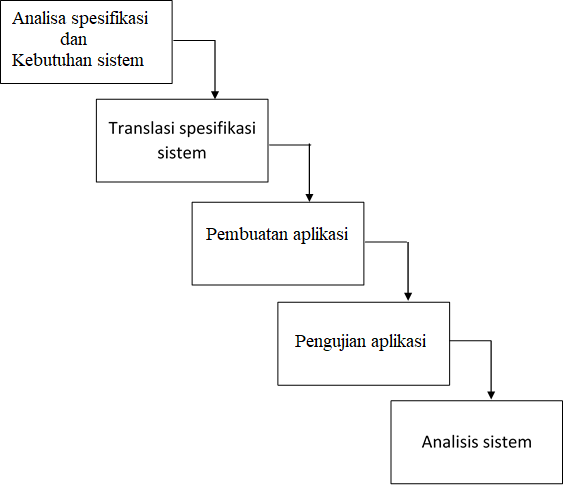
\includegraphics[scale=0.7]{metodologi_proposal}
		
		\caption{Metodologi.}
	\end{centering}
\end{figure}

\section{Analisa spesifikasi dan Kebutuhan sistem}

Menganalisa spesifikasi-spesifikasi pada teka-teki sudoku, lalu membuat kebutuhan dari aplikasi sistem yang akan mengeluarkan \textit{use case} aplikasi.

\section{Translasi spesifikasi sistem}

Aturan-aturan yang telah ditranslasikan dalam CNF di translasikan pada bahasa python dan dibuatkan aturan DIMACSnya seberti berikut:

\begin{enumerate}
	\item Setiap baris memuat bilangan antara 1 
	hingga 9 : 
	
	$\bigwedge_{r=1}^{9}$$\bigwedge_{n=1}^{9}$$\bigvee_{c=1}^{9}$$p\left(r,c,n\right)$
	
	\vspace{5mm}
	
	Skrip python :
	
	\vspace{5mm}
	
	\texttt{def aturan1(dimacs):}
	
	\qquad\qquad\texttt{for r in range(1, 10):}
	
	\qquad\qquad\qquad\texttt{for n in range(1, 10):}
	
	\qquad\qquad\qquad\qquad\texttt{for c in range(1, 10):}
	
	\qquad\qquad\qquad\qquad\qquad\texttt{dimacs += str(r) + str(c) + str(n) + ' 0\textbackslash n'}
	
	\qquad\qquad\qquad\qquad\texttt{global klausa}
	
	\qquad\qquad\qquad\qquad\texttt{klausa += 1}
	
	\qquad\qquad\texttt{return dimacs}
	
	
	\item Setiap kolom memuat bilangan antara 1 hingga 9 : 
	
	$\bigwedge_{c=1}^{9}$$\bigwedge_{n=1}^{9}$$\bigvee_{r=1}^{9}$$p\left(r,c,n\right)$
	
	
	\vspace{5mm}
	
	Skrip python :
	
	\vspace{5mm}
	
	\texttt{def aturan1(dimacs):}
	
	\qquad \qquad\texttt{for c in range(1, 10):}
	
	\qquad \qquad \qquad\texttt{for n in range(1, 10):}
	
	\qquad \qquad \qquad \qquad\texttt{for r in range(1, 10):}
	
	\qquad\qquad\qquad\qquad\qquad\texttt{dimacs += str(r) + str(c) + str(n) + ' 0\textbackslash n'}
	
	\qquad \qquad \qquad \qquad\texttt{global klausa}
	
	\qquad \qquad \qquad \qquad\texttt{klausa += 1}
	
	\qquad \qquad\texttt{return dimacs}
	
	\item Setiap submatriks atau blok $3 \times 3$
	memuat bilangan antara 1 hingga 9 : 
	
	$\bigwedge_{i=0}^{2}$$\bigwedge_{j=0}^{2}$$\bigwedge_{n=1}^{9}$$\bigvee_{r=3i+1}^{3i+3}$$\bigvee_{c=3j+1}^{3j+3}$$p\left(r,c,n\right)$
	
	
	\vspace{5mm}
	
	Skrip python :
	
	\vspace{5mm}
	
	\texttt{def aturan1(dimacs):}
	
	\qquad \qquad\texttt{for i in range(0, 3):}
	
	\qquad \qquad \qquad\texttt{for j in range(0, 3):}
	
	\qquad \qquad \qquad \qquad\texttt{for n in range(1, 10):}
	
	\qquad\qquad\qquad\qquad\qquad\texttt{for r in range(3*i+1, 3*i+4):}
	
	\qquad\qquad\qquad\qquad\qquad\qquad\texttt{for c in range(3*j+1, 3*j+4):}
	
	\qquad\qquad\qquad\qquad\qquad\qquad\qquad\texttt{dimacs += str(r) + str(c) + str(n) + ' 0\textbackslash n'}
	
	\qquad\qquad\qquad\qquad\qquad\qquad\texttt{global klausa}
	
	\qquad\qquad\qquad\qquad\qquad\qquad\texttt{klausa += 1}
	
	\qquad\qquad\texttt{return dimacs}
	
	\vspace{5mm}
	
	Setiap sel memuat paling banyak satu bilangan antara 1 hingga 9 : 
	
	\vspace{5mm}
	
	
	\item Setiap sel memuat paling banyak satu bilangan antara 1 hingga 9 : 
	
	$\bigwedge_{r=1}^{9}$$\bigwedge_{c=1}^{9}$$\bigwedge_{n=1}^{8}$$\bigwedge_{i=n+1}^{9}$
	$\left(\neg p\left(r,c,n\right)\vee\neg p\left(r,c,i\right)\right)$
	
	
	\vspace{5mm}
	
	Skrip python :
	
	\vspace{5mm}
	
	\texttt{def aturan1(dimacs):}
	
	\qquad \qquad\texttt{for e in range(0, 3):}
	
	\qquad \qquad \qquad\texttt{for c in range(0, 3):}
	
	\qquad \qquad \qquad \qquad\texttt{for n in range(1, 9):}
	
	\qquad\qquad\qquad\qquad\qquad\texttt{for i in range(n+1, 10):}
	
	\qquad\qquad\qquad\qquad\qquad\qquad\texttt{dimacs += '-' + str(r) + str(c) + str(n) + ' ' + '-' + str(r) + str(c) + str(i) + ' 0\textbackslash n'}
	
	\qquad\qquad\qquad\qquad\qquad\texttt{global klausa}
	
	\qquad\qquad\qquad\qquad\qquad\texttt{klausa += 1}
	
	\qquad \qquad\texttt{return dimacs}
	
\end{enumerate}

\section{Pembuatan aplikasi}

Spesifikasi yang sudah dalam bentuk CNF akan digunakan pada \textit{SAT Solver}. Lalu \textit{use case} yang didapat akan dibuat fungsionalitasnya. Pembuatan aplikasi menggunakan \textit{waterfall design} tahapan-nya berupa:

\subsection{Spesifikasi Aplikasi}

Spesifikai aplikasi adalah sebagai berikut:
\begin{enumerate}
	\item Bermain sudoku.
	\item Membuat sudoku.
	\item Memecahkan sudoku.
\end{enumerate}

\begin{figure}[H]
	\begin{centering}
		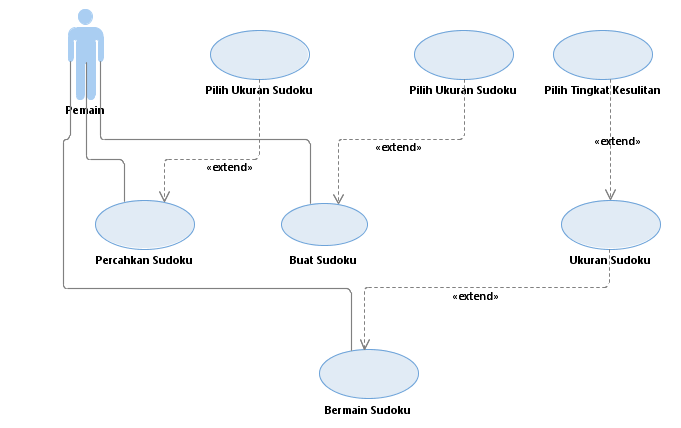
\includegraphics[scale=1]{gambar/useCase}
		
		\caption{\textit{Use Case Diagram}.}
	\end{centering}
\end{figure}

\subsection{\textit{Analysis}}

Dalam \textit{analysis}, penulis menjabarkan mulai dari hal
mendasar yaitu kendala global dalam pengembangan perangkat lunak yang sudah ada. Adapun masalahnya adalah minimnya aplikasi pemecah sudoku yang interaktif.

\subsection{\textit{Design}}

Fitur yang akan ada pada aplikasi tersebut adalah sebagai berikut

 \begin{enumerate}
 	\item Bermain sudoku.
 	\item Membuat sudoku.
 	\item Pecahkan sudoku.
 \end{enumerate}

\subsection{Implementasi}

Lalu dalam tahap \textit{coding} penulis akan menggunakan
bahasa pemograman python dengan SAT \textit{solver} \cite{SATPy2} sebagai dasarnya. Setelah itu akan ditambahkan GUI dan \textit{use case} yang telah di buat.

\section{Pengujian aplikasi}

Pada tahap ini aplikasi akan diujikan kebeberapa penguji dengan diberikan lembat \textit{test case} yang meliputi beberapa aspek kualitas pada aplikasi. Teknik yang digunakan pada pengujian adalah pengujian kotak hitam \cite{TEST1}.

\section{Analisis sistem}

Menganalisa kelayakan kualitas dari aplikasi berdasarkan hasil dari pengujian.
%
%\chapter{Verifikasi Formal dan Analisisnya}

Pada bab ini dijelaskan tentang proses verifikasi formal diagram aktivitas
alur distribusi vaksin menggunakan model checker NuSMV.

\section{Langkah-Langkah Verifikasi Menggunakan NuSMV}

Pada subbab ini, penulis akan menjelaskan cara verifikasi dengan model
checker NuSMV dengan model formal dan spesifikasi yang telah dibuat
pada Bab 3. Berikut langkah verifikasi:
\begin{enumerate}
	\item Buat skrip baru dengan ekstensi .smv menggunakan text editor. Skrip
	tersebut berisi model formal yang telah ditranslasi ke NuSMV pada
	Subbab 3.3.
	\item Tambahkan spesifikasi LTL yang telah dibuat pada Subbab 3.4 dengan
	menyesuaikan aturan pada Bab 2 agar spesifikasi dapat diperiksa
	pada NuSMV.
	\item Simpan skrip ke direktori \texttt{C:/Program Files/NuSMV/<version>/bin}.
	\item Jalankan program Command Prompt. Ubah direktori ke tempat penyimpanan
	skrip yang sudah dibuat.
	\item Masukkan perintah \texttt{NuSMV.exe <namaskrip>.smv} kemudian tekan \textit{enter}.
	\item Hasil verifikasi akan terlihat ketika file NuSMV sudah selesai diproses.
	Jika spesifikasi benar maka NuSMV akan menampilkan spesifikasi is \textit{true}.
	Jika spesifikasi salah maka NuSMV akan menampilkan \textit{counter-example}
	dari spesifikasi tersebut.
\end{enumerate}

\section{Verifikasi Alur Distribusi Vaksin}

Pada Subbab ini akan dijelaskan hasil verifikasi yang dilakukan pada
model formal yang telah dibuat dan analisi dari hasil tersebut.

\subsection{Verifikasi untuk Alur Penerimaan Vaksin}

Berdasarkan spesifikasi yang telah dijelaskan pada Subbab 3.4, didapatkan
hasil verifikasi seperti berikut.

\begin{figure}[H]
	\begin{centering}
		\includegraphics[scale=0.5]{\string"C:/Users/fikri/Google Drive/Tugas_Akhir/assets/verifikasi_nusmv/PenerimaanVaksin\string"}
		\par
	\end{centering}
	
	\caption{Hasil verifikasi untuk alur penerimaan vaksin.}
\end{figure}

Pada Gambar 4.1 terlihat semua spesifikasi bernilai true. Hal itu
menunjukkan bahwa model formal telah memenuhi spesifikasi yang diberikan.

\subsection{Verifikasi untuk Alur Pemeriksaan Vaksin}

Berdasarkan spesifikasi yang telah dijelaskan pada Subbab 3.4, didapatkan
hasil verifikasi seperti berikut:

\begin{figure}[H]
	\begin{centering}
		\includegraphics[scale=0.5]{\string"C:/Users/fikri/Google Drive/Tugas_Akhir/assets/verifikasi_nusmv/PemeriksaanVaksin\string"}
		\par
	\end{centering}
	
	\caption{Hasil verifikasi untuk alur pemeriksaan vaksin.}
	
\end{figure}

Pada Gambar 4.2 terlihat semua spesifikasi bernilai true. Hal itu
menunjukkan bahwa model formal telah memenuhi spesifikasi yang diberikan.

\subsection{Verifikasi untuk Alur Cek Prioritas Pengiriman}

Berdasarkan spesifikasi yang telah dijelaskan pada Subbab 3.4, didapatkan
hasil verifikasi seperti berikut:

\begin{figure}[H]
	\begin{centering}
		\includegraphics[scale=0.5]{\string"C:/Users/fikri/Google Drive/Tugas_Akhir/assets/verifikasi_nusmv/CekPrioritasPengiriman\string"}
		\par
	\end{centering}
	
	\caption{Hasil verifikasi untuk alur cek prioritas pengiriman.}
\end{figure}

Pada Gambar 4.3 terlihat semua spesifikasi bernilai true. Hal itu
menunjukkan bahwa model formal telah memenuhi spesifikasi yang diberikan.

\subsection{Verifikasi untuk Alur Penyimpanan di PT. Bio Farma}

Berdasarkan spesifikasi yang telah dijelaskan pada Subbab 3.4, didapatkan
hasil verifikasi seperti berikut:

\begin{figure}[H]
	\begin{centering}
		\includegraphics[scale=0.5]{\string"C:/Users/fikri/Google Drive/Tugas_Akhir/assets/verifikasi_nusmv/BioFarma-01\string"}
		\par
	\end{centering}
	
	\caption{Hasil verifikasi untuk alur penyimpanan di PT. Bio Farma.}
	
\end{figure}

\begin{figure}[H]
	\begin{centering}
		\includegraphics[scale=0.5]{\string"C:/Users/fikri/Google Drive/Tugas_Akhir/assets/verifikasi_nusmv/BioFarma-02\string"}
		\par
	\end{centering}
	
	\caption{Hasil verifikasi untuk alur penyimpanan di PT. Bio Farma.}
	
\end{figure}

Pada Gambar 4.4 dan 4.5 terdapat spesifikasi yang bernilai false yaitu
\texttt{F(ac = hubungi$\_$supervisor) xor F(ac = pengiriman$\_$vaksin)}. Hal itu
menunjukkan bahwa petugas vaksin tidak akan menghubungi supervisor atau
vaksin tidak akan dikirim ke pos selanjutnya. Berdasarkan counterexample
yang diberikan oleh NuSMV, pada model formal terdapat proses yang
terus-menerus terjadi. Proses tersebut terjadi ketika \texttt{pemeriksaan\_vaksin} dan \texttt{cek\_jadwal\_ pengiriman} terus-menerus dilakukan. Data yang
didapat dari BPOM dan WHO tidak ada informasi yang menjelaskan berapa
lama waktu vaksin disimpan di ruang penyimpanan.

\subsection{Verifikasi untuk Alur Penyimpanan di Dinas Kesehatan}

Berdasarkan spesifikasi yang telah dijelaskan pada Subbab 3.4, didapatkan
hasil verifikasi seperti berikut.

\begin{figure}[H]
	\begin{centering}
		\includegraphics[scale=0.5]{\string"C:/Users/fikri/Google Drive/Tugas_Akhir/assets/verifikasi_nusmv/DinKes-01\string"}
		\par
	\end{centering}
	
	\caption{Hasil verifikasi untuk alur penyimpanan di Dinas Kesehatan.}
	
\end{figure}

\begin{figure}[H]
	\begin{centering}
		\includegraphics[scale=0.5]{\string"C:/Users/fikri/Google Drive/Tugas_Akhir/assets/verifikasi_nusmv/DinKes-02\string"}
		\par
	\end{centering}
	
	\caption{Hasil verifikasi untuk alur penyimpanan di Dinas Kesehatan.}
	
\end{figure}

Pada Gambar 4.6 dan 4.6 terdapat spesifikasi yang bernilai false yaitu \texttt{F(ac = hubungi$\_$supervisor) xor F(ac = pengirimanan$\_$vaksin)}. Hal itu menunjukkan bahwa petugas vaksin tidak akan menghubungi superviosr atau vaksin tidak akan dikirim ke pos selanjutnya. Berdasarkan \textit{counterexample} yang diberikan oleh NuSMV, pada model formal terdapat proses yang terus-menerus terjadi. Proses tersebut terjadi ketika \texttt{pemeriksaan\_vaksin} dan \texttt{cek\_jadwal\_ pengiriman} terus-menerus dilakukan. Data yang didapat dari BPOM dan WHO tidak ada informasi yang menjelaskan berapa lama waktu vaksin disimpan di ruang penyimpanan.

\subsection{Verifikasi untuk Alur Penyimpanan di Puskesmas}

Berdasarkan spesifikasi yang telah dijelaskan pada Subbab 3.4, didapatkan
hasil verifikasi seperti berikut.

\begin{figure}[H]
	\begin{centering}
		\includegraphics[scale=0.5]{\string"C:/Users/fikri/Google Drive/Tugas_Akhir/assets/verifikasi_nusmv/Puskesmas-01\string"}
		\par
	\end{centering}
	
	\caption{Hasil verifikasi untuk alur penyimpanan di Puskesmas.}
	
\end{figure}

\begin{figure}[H]
	\begin{centering}
		\includegraphics[scale=0.5]{\string"C:/Users/fikri/Google Drive/Tugas_Akhir/assets/verifikasi_nusmv/Puskesmas-02\string"}
		\par
	\end{centering}
	
	\caption{Hasil verifikasi untuk alur penyimpanan di Puskesmas.}
	
\end{figure}

Pada Gambar 4.8 dan 4.9 terdapat spesifikasi yang bernilai false yaitu
\texttt{F(ac = hubungi$\_$supervisor) xor F(ac = imunisasi)}. Hal itu
menunjukkan bahwa petugas vaksin tidak akan menghubungi supervisor atau
vaksin tidak akan dikirim ke pos selanjutnya. Berdasarkan counterexample
yang diberikan oleh NuSMV, pada model formal terdapat proses yang
terus-menerus terjadi. Proses tersebut terjadi ketika \texttt{pemeriksaan\_vaksin} dan \texttt{cek\_jadwal\_imunisasi} terus-menerus dilakukan. Data yang
didapat dari BPOM dan WHO tidak ada informasi yang menjelaskan berapa
lama waktu vaksin disimpan di ruang penyimpanan.
%
%\chapter{Kesimpulan dan Saran}

Pada bab ini dijelaskan kesimpulan dari pengerjaan tugas akhir dan saran untuk penelitian selanjutnya.

\section{Kesimpulan}

Berikut adalah kesimpulan yang didapat dari pengerjaan tugas akhir yang telah dilakukan:

\begin{enumerate}
	\item Deskripsi alur distribusi vaksin di Indonesia yang diberikan oleh PT. Bio Farma memenuhi persyaratan keamanan yang ditentukan oleh BPOM dan WHO.
	
	\item Deskripsi alur distribusi vaksin di Indonesia yang diberikan oleh PT. Bio Farma tidak cukup rinci untuk memenuhi persyaratan fungsional tambahan, yaitu persyaratan fungsional tambahan pada alur penyimpanan di PT. Bio Farma, Dinas Kesehatan, dan Puskesmas. Ini berarti terdapat kondisi pada alur penyimpanan di PT. Bio Farma, Dinas Kesehatan, dan Puskesmas yang menyebabkan vaksin tidak dikirim atau petugas vaksin menghubungi supervisor.
	
	\item Berdasarkan hasil verifikasi pada Bab 4, metode formal dapat melakukan verifikasi pada alur distribusi dan dapat menemukan kesalahan pada model yang telah dibuat.
	
\end{enumerate}

\section{Saran}

Berikut adalah saran-saran untuk penilitian selanjutnya:

\begin{enumerate}
	\item Berdasarkan hasil verifikasi pada Bab 4, diagram aktivitas belum dapat merepresentasikan secara rinci alur distribusi vaksin. Oleh karena itu, peneliti selanjutnya dapat menggunakan model lain yang lebih detail dan bervariasi, seperti dapat menangani masalah waktu.
	
	\item Pada penelitian selanjutnya, sebaiknya menggunakan bahasa formal lain agar spesifikasi formal yang akan diverifikasi dapat lebih detail.
\end{enumerate}
%
\cleardoublepage
\addcontentsline{toc}{chapter}{Daftar Pustaka}
\bibliographystyle{IEEEtran} %harvard style
\bibliography{References}
%
%\pagebreak
\cleardoublepage
\addcontentsline{toc}{chapter}{Lampiran}
\chapter*{Lampiran}

Pada bab ini akan berisi lampiran dari pengerjaan tugas akhir.
\end{document}
